% Template LaTeX document for CSSR4Africa Deliverables
% Adapted from documents prepared by EPFL for the RobotCub project
% and subsequently by the University of Skövde for the DREAM project
%
% DV 28/06/2023

\documentclass{CSSRforAfrica}

\usepackage[titletoc,title]{appendix}
\usepackage[colorlinks, urlcolor=blue, linkcolor=black, citecolor=black]{hyperref}
\usepackage{latexsym}
\usepackage{comment}
\usepackage{multirow}
\usepackage{subcaption}
\usepackage[breakable,skins,most]{tcolorbox} % Consolidated tcolorbox options
\usepackage{tabularx,colortbl}
\usepackage[tikz]{bclogo} % for boxes
\usepackage{ragged2e}
\usepackage{dirtree}
\usepackage{listings}
\usepackage{textcomp}
\usepackage{natbib}
\usepackage{url}
\usepackage{graphicx}
\usepackage{array}
\usepackage{longtable}
\usepackage{enumitem}



%%% for listing %%%%%%%%%%%%%%%%%%%%%%%%%%%%%%
\captionsetup[figure]{format=hang}
\usepackage{xcolor}
\definecolor{codegreen}{rgb}{0,0.6,0}
\definecolor{codegray}{rgb}{0.5,0.5,0.5}
\definecolor{codepurple}{rgb}{0.58,0,0.82}
\definecolor{backcolour}{rgb}{0.95,0.95,0.92}
\definecolor{greenyellow}{rgb}{0.8, 0.7, 0.10} % Example values, adjust as needed

\lstdefinestyle{withoutNumbering}{
	backgroundcolor=\color{backcolour},   
	commentstyle=\color{codegreen},
	keywordstyle=\color{magenta},
	stringstyle=\color{codepurple},
	basicstyle=\ttfamily\small,
	breakatwhitespace=false,         
	breaklines=true,                 
	captionpos=b,                    
	keepspaces=true,                 
	showspaces=false,                
	showstringspaces=false,
	showtabs=false,                  
	tabsize=2
}
%%%%%%%%%%%%%%%%%%%%%%%%%%%%%%%%%%%%%%%%%%%%%%%%%%%
\definecolor{backcolour}{rgb}{0.95,0.95,0.95}
\definecolor{irongray}{HTML}{6D6E71}
\definecolor{LightGray}{gray}{0.9}

\newcommand{\blank}{~\\}
\newcommand{\checkbox}{{~~~~~~~\leavevmode \put(-7,-1.5){  \huge $\Box$  }}}

\begin{document}
\input{epsf}

%%
%% SHOULD NOT NEED TO BE CHANGED BEFORE THIS POINT
%% ------------------------------------------------
%%


\deliverable{D4.1}         
\title{D4.1 Sensor Tests}   

\leadpartner{Carnegie Mellon University Africa} % REPLACE with partner name: Carnegie Mellon University Africa or The University of the Witwatersrand
\partner{}                                      

\revision{1.1}                           
\deliverabledate{1/10/2023}    
\submissiondate{26/03/2024}   
\revisiondate{31/05/2025}   
\disseminationlevel{PU}
\responsible{Yohannes Haile}  


%%
%% Create the titlepage
%%

\maketitle
 

\section*{Executive Summary}
%===============================================================
\label{executive_summary}
%%\addcontentsline{toc}{section}{Executive Summary}
 
Deliverable D4.1 aims to create a robust suite of unit tests to verify that sensor data is successfully 
acquired on each sensor topic. The key components of this deliverable include a ROS node called 
\texttt{sensorTest}, a report documenting the development process, requirements refinement and 
specifying functional characteristics, and a user manual on how to build and launch the module. 
The interface design encompasses input, output, and control data. Suitable data structures are 
specified, and coding adheres to software engineering standards. 

\newpage
 
 
\pagebreak
\tableofcontents
\newpage


\section{Introduction}
%===============================================================
This deliverable is dedicated to ensuring the optimal functionality of the sensors on the 
Pepper robot (or simulator), with a primary focus on verifying their ability to successfully 
acquire data from their designated topics. Illustrated in Figure \ref{fig: Pepper robot sensor},
the diverse array of sensors on Pepper plays a critical role in shaping its perception and 
interactive capabilities.

At the core of Pepper's visual perception are the dual RGB cameras, functioning as its primary 
set of visual sensors. These cameras capture images with a broad range of resolutions, offering 
Pepper a comprehensive view from two distinct fields of vision. Working in tandem with the RGB 
cameras, the depth sensor enriches Pepper's spatial understanding by providing essential 
information about the distance to objects in its environment. The microphones are equipped 
to give Pepper auditory perception capabilities. This feature is pivotal for speech recognition, 
sound detection, and localization which facilitates effective communication with users. 

Supplementing Pepper's tactile interaction capabilities are the touch sensors distributed in 
the head and hand sensor areas. These sensors enhance the robot's ability to engage naturally 
with humans and its surroundings, fostering interactive and intuitive experiences. The sonar 
sensor further contributes to Pepper's environmental awareness by gauging distances to nearby 
objects, proving integral to tasks such as navigation, obstacle avoidance, and maintaining 
spatial awareness during movement.

For Pepper's physical coordination, the gyroscope and accelerometer sensors are used to detect 
changes in orientation and acceleration respectively. This information is vital for 
the robot to maintain balance and coordination across a spectrum of activities. 
Additionally, the laser sensor introduces another layer to Pepper's environmental 
perception, emitting laser beams and measuring their reflections. 

\begin{figure}[!hbpt]
	\centering
	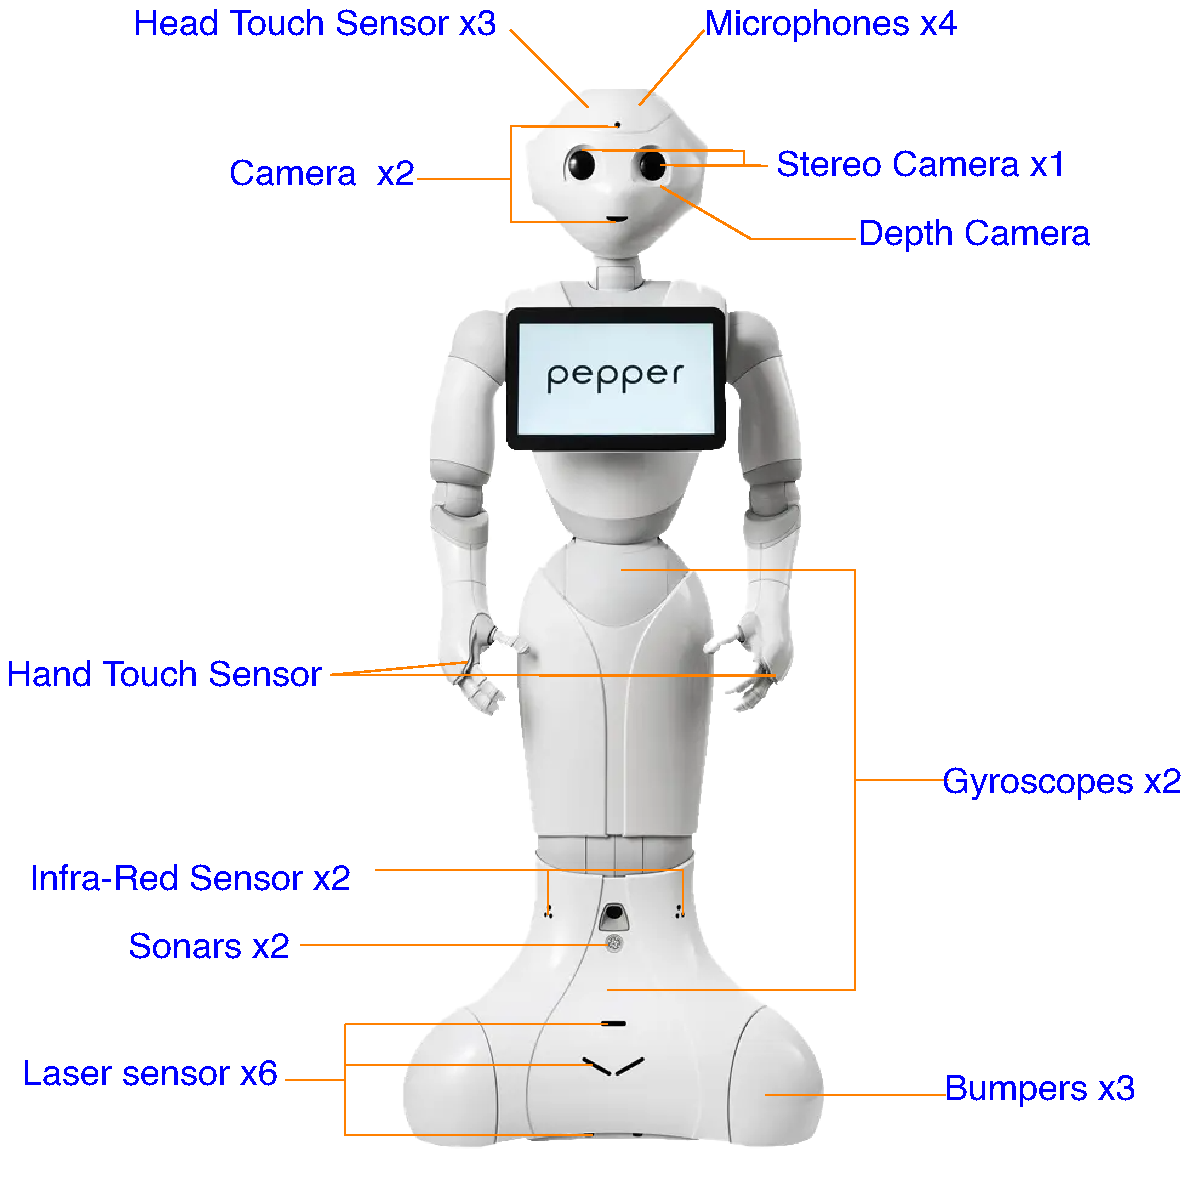
\includegraphics[scale=0.51]{images/Pepper_Sensor.pdf}
	\caption{Pepper robot sensors}
	\label{fig: Pepper robot sensor}
\end{figure}

The ROS-NAOqi driver provides a bridge between ROS(Robot Operating System) and NAOqiOS, 
the operating system of Aldebaran's Nao, Pepper, and Romeo robots \cite{SoftBankDocumentation}. 
The driver publishes all sensor and actuator data as well as basic diagnostic information 
for battery and temperature. It also subscribes to RViz and cmd\_vel for teleportation. 
The ROS-NAOqi Interface comprises ROS nodes that interact with NAOqi via the NAOqi messaging 
API. These nodes can subscribe to and publish ROS topics, facilitating communication 
with other ROS nodes.

\newpage

\section{Requirements Definition}
The sensor test provides a systematic process aimed at understanding and documenting the
functionality needs that the module must fulfill. This deliverable is important in identifying 
the specific users expectations, ensuring that the module will be capable of performing the precise
sensor tests in various scenarios and environments. The test encompasses a thorough examination of the 
intended functionality, the user's needs, and the project's objectives to ensure that the module 
will meet the requirements of the project. 

As seen from the diagram in Figure \ref{fig: Pepper robot sensor}, the Pepper robot is equipped with
a variety of sensors that are essential for its operation. For this deliverable,
the camera sensors will be tested to ensure that they can capture images and videos. 
The depth sensor will be tested to ensure that it can capture depth information. The 
microphone sensor will be tested to ensure that it can capture audio data. The IMU sensor 
will be tested to ensure that it can capture orientation and acceleration data. The sonar 
sensor will be tested to ensure that it can capture distance data. The laser sensor will 
be tested to ensure that it can capture distance data. The odometry sensor will be tested 
to ensure that it can capture odometry data. The joint states sensor will be tested to 
ensure that it can capture joint state data for the joint actuator of the robot. 
Exceptionally, the loudspeaker, even though it is not a sensor, will be tested to ensure that it
can speak out the text provided to it.

\subsection*{Misalignment of the Module}
Due to the unavailability of the head touch, hand touch, and bumper sensors, the module will not 
be able to test these sensors. Given the current status of the project, we have opted to suspend 
work on it, as we have not identified a direct application for these sensors. However, should the
future direction of our project necessitate the integration of these sensors due to their potentially
critical role, we will undertake efforts to ensure their functionality.

In regards to the sensor test for the simulator, the microphone sensor, IMU, stereo camera, and loudspeaker
test will not be conducted as they are not available in the simulator. Furthermore, the Gazebo simulator 
will raise errors when testing for the camera is conducted in parallel mode. Therefore, the camera sensors 
should be tested in sequential mode.
\newpage

\section{Module Specifications}
To validate the functionality of the sensors, the sensor test module is designed to execute a series of tests
on the sensors. The sensor test module is a ROS node that subscribes to the sensor topics and verifies that the
sensors can capture data. The sensor test module is designed to test the following 


% Itemize the sensors that will be tested
\begin{itemize}
	\setlength\itemsep{0em}
	\item Back Sonar
	\item Front Sonar
	\item Bottom Camera
	\item Front Camera
	\item Depth Camera
	\item Stereo Camera \textbf{\textit{(not available in the simulator)}}
	\item Realsense RGB Camera \textbf{\textit{(not available in the simulator)}}
	\item Realsense Depth Camera \textbf{\textit{(not available in the simulator)}}
	\item Laser Sensor
	\item Microphone \textbf{\textit{(not available in the simulator)}}
	\item Joint State
	\item Odometry
	\item IMU \textbf{\textit{(not available in the simulator)}}
	\item Speech (Loudspeaker) \textbf{\textit{(not available in the simulator)}}
\end{itemize}

All of the sensors will be tested for 10 seconds, whereas the microphone sensor will be tested for a total of 40 seconds, where each microphone will be tested for 10 seconds.
For the loudspeaker, a text will passed on it to speak out. The sensor test will be conducted in two modes: parallel and sequential.
In the parallel mode, all the sensors will be tested at the same time, whereas in the sequential mode, the sensors will be tested one after the other.
The sensor test will be conducted for both the robot and the simulator.

To test the sensors, the sensor test module will read various configuration files that contain the necessary information for the test.
The configuration files include the sensor test configuration file, the sensor test input file, and the topics file. The sensor test configuration file
contains the platform to be tested, the mode of the test, and the topics file for the robot and simulator. The sensor test input file contains the sensors to be tested.
The topics file contains the list of topics for the robot and simulator. The sensor test module will publish the results of the test to the sensor test output file.
Furthermore, the sensor test module will record the video and audio data for the camera and microphone sensors respectively, and store them in the data directory as specified 
by the user in the \texttt{sensorTestImplementation.cpp} file.

\newpage

\section{Interface Design}
\subsection*{File Structure and Organization}
The source code for conducting sensor tests is structured into two primary components: \\
\texttt{sensorTestApplication} and 
\texttt{sensorTestImplementation}. The sensorTestImplementation component encapsulates all the essential functionality 
required for executing comprehensive sensor tests. This includes all of the tests for the sensors that 
consist of the bottom, front, and stereo camera, depth camera, sonar, laser, odom, microphone, speech, and joint states. 
In addition to sensor testing capabilities, this component is also equipped with the functionality to process various files 
critical for the testing process, such as configuration files, input files, and topics files.

On the other hand, the sensorTestApplication invokes those functions for the testing process. It is tasked with 
executing functions defined within the sensorTestImplementation, effectively managing the sensor test operations.\\

Here is the file structure of the pepper interface tests package:
\vspace{0.5cm}

\renewcommand*\DTstyle{\ttfamily}
\dirtree{%
	.1 pepper\_interface\_tests.
	.2 config.
	.3 actuatorTestConfiguration.ini.
	.3 actuatorTestInput.ini.
	.3 sensorTestInput.ini.
	.3 sensorTestConfiguration.ini.
	.2 data.
	.3 pepperTopics.dat.
	.3 sensorTestOutput.dat.
	.3 simulatorTopics.dat.
	.2 include.
	.3 pepper\_interface\_tests.
	.4 actuatorTestInterface.h.
	.4 sensorTestInterface.h.
	.2 launch.
	.3 actuatorTestLaunchRobot.launch.
	.3 sensorTestLaunchRobot.launch.
	.3 interfaceTestLaunchSimulator.launch.
	.2 src.
	.3 actuatorTestApplication.cpp.
	.3 actuatorTestImplementation.cpp.
	.3 sensorTestApplication.cpp.
	.3 sensorTestImplementation.cpp.
	.2 README.md.
	.2 CMakeLists.txt.
	.2 package.xml.
}

\subsection*{Configuration File}
The operation of the \texttt{sensorTest} node is determined by the contents of the configuration file that contains a list of key-value pairs as shown below. 

The configuration file is named \texttt{sensorTestConfiguration.ini}

% Table of 3 x 4 with the following headers: Key, Value, Description
\begin{longtable}[c]{|l|l|p{7cm}|}
	\caption{Configuration file for the sensor test.} \label{tab:config_file}\\
	\hline
	\rowcolor{gray!30}
	\small{\textbf{Key}} & \small{\textbf{Value}} & \small{\textbf{Description}} \\ \hline
	\endhead % header for subsequent pages
	
	\small{\texttt{platform}} & \small{\texttt{simulator}} or \texttt{robot} & \small{Specifies the platform to be tested. The platform can be set to either \texttt{simulator} or \texttt{robot}.} \\ \hline
	\small{\texttt{robotTopics}} & \small{\texttt{robotTopics.dat}} & \small{Specifies the name of the robot topics file. The robot topics file contains the list of topics for the robot.} \\ \hline
	\small{\texttt{simulatorTopics}} & \small{\texttt{simulatorTopics.dat}} & \small{Specifies the name to the simulator topics file. The simulator topics file contains the list of topics for the simulator.} \\ \hline
	\small{\texttt{mode}} & \small{\texttt{parallel}} or \texttt{sequential} & \small{Specifies the mode of the test. The mode can be either \texttt{parallel} or \texttt{sequential}. The parallel mode runs all the tests in parallel. The sequential mode runs all the tests sequentially.} \\ \hline
	
\end{longtable}

\subsection*{Input File}
The input file is used to specify which sensors to test by using the sensor name as the key and \texttt{True} or \texttt{False} as the value. 
The sensor name must be the same as the sensor name in the topics file. 

The input file is named \texttt{sensorTestInput.ini}

\subsection*{Output Data File}

The output data file is used to store the results of the sensor tests. The output data file is written in the \texttt{.dat} file format.  
It logs relevant information such as sensor names, image resolutions, encodings, and test results. The specific content depends on the type of sensor being tested.

The detailed structure and examples of the output file are provided in the \textit{Results} section.

The output data file is named \texttt{sensorTestOutput.dat}.

Furthermore, the recorded video and audio files are stored in the \texttt{data} directory. These files include:

\begin{itemize}[itemsep=1pt, parsep=0pt]
	\item \texttt{frontCameraOutput.mp4}
	\item \texttt{bottomCameraOutput.mp4}
	\item \texttt{stereoCameraOutput.mp4}
	\item \texttt{depthCameraOutput.mp4}
	\item \texttt{realsenseRGBOutput.mp4}
	\item \texttt{realsenseDepthOutput.mp4}
	\item \texttt{microphoneOutput.wav}
\end{itemize}


Each file corresponds to a specific sensor and is used for offline analysis and documentation of the test results.

\subsection*{Topics File}
For the test, a selected list of the topics for the robot and simulator is stored in the topics file. The topic files are written in the .dat file format. 
The data file is written in key-value pairs where the key is the sensor name and the value is the topic 

The topics file for the robot is named \texttt{robotTopics.dat} and the topics file for the simulator is named \texttt{simulatorTopics.dat}

\subsubsection*{Topics Subscribed}
The sensorTest node subscribes to the following topics:
\begin{longtable}[c]{|p{8cm}|p{4.2cm}|l|}
	\caption{Topics subscribed by the sensorTest node.} \label{tab:subscribed_topics}\\
	\hline
	\rowcolor{gray!30}
	\small{\textbf{Topic}} & \small{\textbf{Sensor}} & \small{\textbf{Platform}} \\ \hline
	\endhead % header for subsequent pages
	
	\small{\texttt{/naoqi\_driver/camera/bottom/image\_raw}} & \small{\texttt{Bottom Camera}} & \small{\texttt{robot}} \\ \hline
	\small{\texttt{/naoqi\_driver/camera/depth/image\_raw}} & \small{\texttt{Depth Camera}} & \small{\texttt{robot}} \\ \hline
	\small{\texttt{/naoqi\_driver/camera/front/image\_raw}} & \small{\texttt{Front Camera}} & \small{\texttt{robot}} \\ \hline
	\small{\texttt{/naoqi\_driver/camera/stereo/image\_raw}} & \small{\texttt{Stereo Camera}} & \small{\texttt{robot}} \\ \hline
	\small{\texttt{/camera/color/image\_raw}} & \small{\texttt{RealSenseCameraRGB}} & \small{\texttt{robot}} \\ \hline
	\small{\texttt{/camera/aligned\_depth\_to\_color/image\_raw}} & \small{\texttt{RealSenseCameraDepth}} & \small{\texttt{robot}} \\ \hline
	\small{\texttt{/naoqi\_driver/audio}} & \small{\texttt{Microphone}} & \small{\texttt{robot}} \\ \hline
	\small{\texttt{/naoqi\_driver/imu/base}} & \small{\texttt{IMU Sensor}} & \small{\texttt{robot}} \\ \hline
	\small{\texttt{/naoqi\_driver/sonar/front}} & \small{\texttt{Sonar Sensor}} & \small{\texttt{robot}} \\ \hline
	\small{\texttt{/naoqi\_driver/sonar/back}} & \small{\texttt{Sonar Sensor}} & \small{\texttt{robot}} \\ \hline
	\small{\texttt{/naoqi\_driver/laser}} & \small{\texttt{Laser}} & \small{\texttt{robot}} \\ \hline
	\small{\texttt{/naoqi\_driver/odom}} & \small{\texttt{Odometry}} & \small{\texttt{robot}} \\ \hline
	\small{\texttt{/joint\_states}} & \small{\texttt{Joint States}} & \small{\texttt{robot}} \\ \hline
	\small{\texttt{/pepper/sonar\_back}} & \small{\texttt{Back Sonar}} & \small{\texttt{simulator}} \\ \hline
	\small{\texttt{/pepper/sonar\_front}} & \small{\texttt{Front Sonar}} & \small{\texttt{simulator}} \\ \hline
	\small{\texttt{/pepper/camera/bottom/image\_raw}} & \small{\texttt{Bottom Camera}} & \small{\texttt{simulator}} \\ \hline
	\small{\texttt{/pepper/camera/depth/image\_raw}} & \small{\texttt{Depth Camera}} & \small{\texttt{simulator}} \\ \hline
	\small{\texttt{/pepper/camera/front/image\_raw}} & \small{\texttt{Front Camera}} & \small{\texttt{simulator}} \\ \hline
	\small{\texttt{/pepper/laser\_2}} & \small{\texttt{Laser}} & \small{\texttt{simulator}} \\ \hline
	\small{\texttt{/pepper/odom}} & \small{\texttt{Odometry}} & \small{\texttt{simulator}} \\ \hline
	\small{\texttt{/joint\_states}} & \small{\texttt{Joint States}} & \small{\texttt{simulator}} \\ \hline
	
\end{longtable}

\subsubsection*{Topics Published}
As explained earlier, the speech topic is listed under the sensor topics because its topic is available under the NAOqi driver sensor topics. The sensorTest node publishes the following topics:
% table of 2 x 3 with the following headers: topic, sensor, platform
% just for speech.
\begin{longtable}[c]{|p{8cm}|p{4cm}|p{1.7cm}|}
	\caption{Topics published by the sensorTest node.} \label{tab:published_topics}\\
	\hline
	\rowcolor{gray!30}
	\small{\textbf{Topic}} & \small{\textbf{Actuator}} & \small{\textbf{Platform}} \\ \hline
	\endhead % header for subsequent pages
	
	\small{\texttt{/speech}} & \small{\texttt{Speakers}} & \small{\texttt{robot}} \\ \hline
	
\end{longtable}


\subsection*{Launch File}
The launch file is used to launch the sensor test. \texttt{sensorTestLaunchRobot.launch} file is used for the robot and \texttt{sensorTestLaunchSimulator.launch} for the simulator. 
The launch file has the following parameters:
\begin{itemize}
	\setlength\itemsep{0em}
	\item \texttt{robot\_ip}: specifies the IP address of the robot.
	\item \texttt{roscore\_ip}: specifies the IP address of the roscore.
	\item \texttt{network\_interface}: specifies the network interface name.
\end{itemize}

A default value is provided for each parameter in the launch file. For the robot\_ip, the default value is 
\texttt{172.29.111.230} and for the network\_interface, the default value is \texttt{eth0}. The roscore\_ip 
parameter can be specified by the user as identified using \texttt{ifconfig} command. But the default value works
hence the user can skip specifying the roscore\_ip parameter. If the user has a different network\_interface name, the user
can change the default value specified in the launch file. 

Three nodes are launched in the launch file: \texttt{naoqi\_driver\_node}, \texttt{naoqiAudio}, and \\
\texttt{naoqiAudioPublisher}. 
The \texttt{naoqi\_driver\_node} is primarily responsible for publishing sensor data from the robot to various topics, 
excluding audio data. For audio data acquisition, the \texttt{naoqiAudio} node is introduced. This node leverages the Python SDK 
to capture audio data directly from the robot. Due to compatibility issues, as the Python SDK operates under 
Python 2 which is not directly integrable with ROS-Noetic which runs Python 3. The \texttt{naoqiAudioPublisher} node bridges this gap through 
the use of web sockets, facilitating the transfer of audio data from the SDK to ROS. This node plays a crucial role 
in processing the audio data by deinterleaving it and then publishing the processed audio to the \texttt{/naoqi\_driver/audio} topic. 

\newpage

The diagram below shows the data flow of the sensor test.
\begin{figure}[!hbpt]
	\centering
	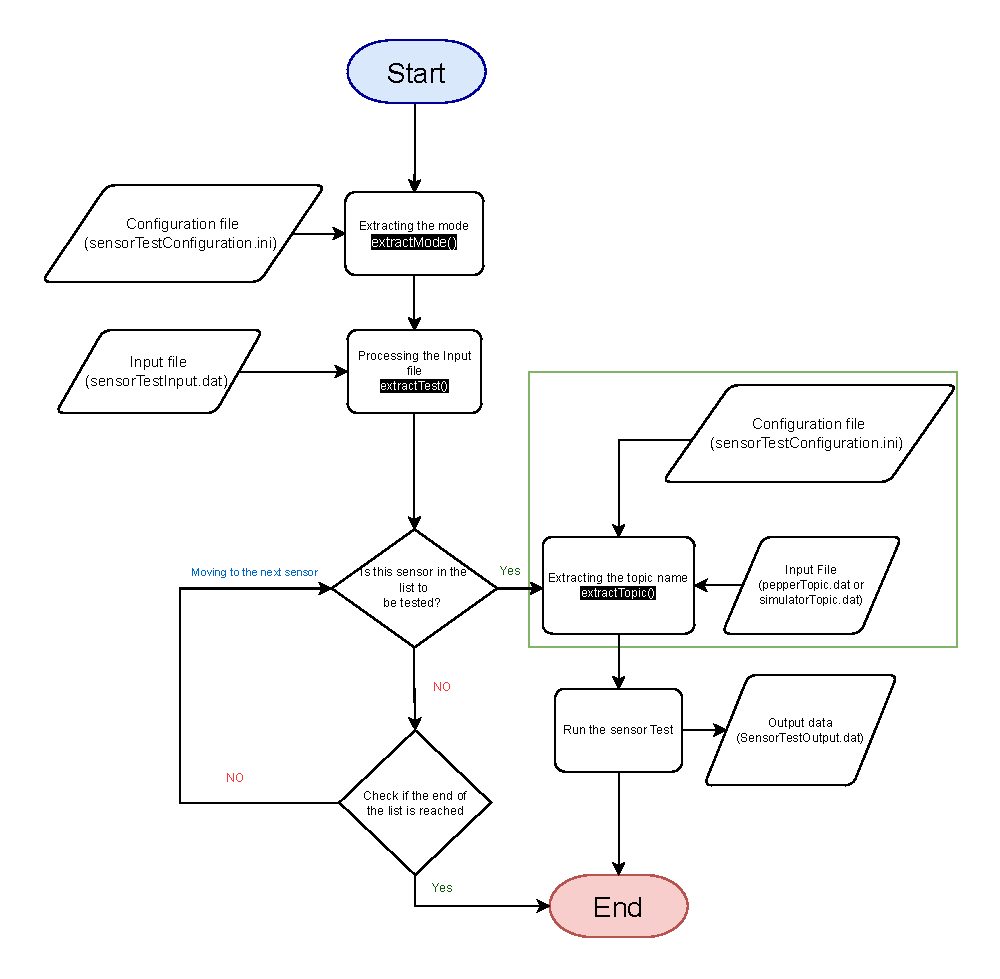
\includegraphics[scale=1.0]{images/Sensor_diagram.pdf}
	\caption{Data Flow Diagram of the Sensor Test.}
	\label{fig: Sensor Test Flow diagram}
\end{figure}

\newpage

\section{Module Design}
For testing the physical robot, the NAOqi driver is used to subscribe to the sensor topics. The  driver provides a hardware interface to connect to 
Aldebaran Nao, Romeo, and Pepper robot. The module first reads the configuration file to get the mode of the test, the platform to be tested, 
and the topics file for the robot. The module then reads the input file to get the sensors to be tested. The module then reads the topics file to get the
topics for the robot. The module then subscribes to the topics for the robot and tests the sensors. 

For the sonar sensor, the module subscribes to the sonar topics. The module then verifies that the sonar sensor can capture distance data. The 
module then logs the distance data to the output data file. For testing the sonar it uses \texttt{sensor\_msgs/Range} message type. This message type 
represents a standardized way to express distance measurements typically gathered from range-sensing devices such as sonar, infrared(IR) sensors, and lidar. 

For the camera sensors, the module subscribes to the camera topics. The module then verifies that the camera sensor can capture image data. The
module then logs the image data to the output data file. For testing the camera sensors, it uses the \texttt{sensor\_msgs/Image} message type. The video data is recorded and stored in the data directory using the \texttt{cv::VideoWriter} class from the 
OpenCV library.

For the depth camera sensor, the module subscribes to the depth camera topic. The module then verifies that the depth camera sensor can capture image data. The
module then logs the image data to the output data file. For testing the depth camera sensor, it uses the \texttt{sensor\_msgs/Image} message type. The video data is recorded and stored in the data directory using the \texttt{cv::VideoWriter} class from the OpenCV library.

For the laser sensor, the module subscribes to the laser topics. The module then verifies that the laser sensor can capture distance data. The
module then logs the distance data to the output data file. For testing the laser sensor, it uses the \texttt{sensor\_msgs/LaserScan} message type. This message type
represents a 1D scan from a planar laser range-finder.

For the microphone sensor, the module subscribes to the audio topic. The module then verifies that the microphone sensor can capture audio data. For testing the 
microphone sensor, it uses a custom message type named \texttt{naoqi\_driver/AudioCustomMsg}. This message type represents audio data for the four microphones of the Pepper 
robot. The audio data is recorded and stored in the data directory. The audio is recorded using \texttt{.wav} format. 

For the joint state sensor, the module subscribes to the joint state topics. The module then verifies that the joint state sensor can capture joint state data. The
module then logs the joint state data to the output data file. For testing the joint state sensor, it uses the \texttt{sensor\_msgs/JointState} message type. This message type
represents the state of the robot's joints.

For the odometry sensor, the module subscribes to the odometry topics. The module then verifies that the odometry sensor can capture odometry data. The
module then logs the odometry data to the output data file. For testing the odometry sensor, it uses the \texttt{nav\_msgs/Odometry} message type. This message type
represents the odometry data for the robot.

For the IMU sensor, the module subscribes to the IMU topics. The module then verifies that the IMU sensor can capture IMU data. The
module then logs the IMU data to the output data file. For testing the IMU sensor, it uses the \texttt{sensor\_msgs/Imu} message type. This message type
represents the IMU data for the robot.

For the speech, the module publishes the text to the speech topic. The module then verifies that the speech can speak out the text. The
module then logs the text to the output data file. For testing the speech, it uses the \texttt{std\_msgs/String} message type that represents a string message.

\newpage


\section{Executing the Sensor Test}
To start the sensor test, the user must first install the necessary software packages as outlined in \href{https://cssr4africa.github.io/deliverables/CSSR4Africa_Deliverable_D3.3.pdf}
{Deliverable D3.3}. Furthermore, you can refer to how to get the parameters for the robot IP, roscore IP, and network interface from Deliverable D3.3.
Referring to the interface section, the user must set the platform to be tested, and specify which mode to run the test. Then using key-value pairs, the user must 
specify which sensors to test by using the sensor name as the key and \texttt{True} or \texttt{False} as the value. 


To launch the sensor test, the user must run the following command:

\begin{lstlisting}[style=withoutNumbering, language=bash]
# Launch the sensors for the physical robot
roslaunch pepper_interface_tests sensorTestLaunchRobot.launch \
robot_ip:=<robot_ip> roscore_ip:=<roscore_ip> \
network_interface:=<network_interface_name>

# Launch the interfaceTestLaunchSimulator for the simulator
roslaunch pepper_interface_tests interfaceTestLaunchSimulator.launch
\end{lstlisting}

The above commands will launch the sensor test for the robot and simulator. 

It's important to note that the tests for actuators and sensors are designed to function autonomously, allowing for the execution of sensor tests 
without necessitating the robot's activation. However, when conducting these tests in a sleep state, the robot's camera will orient downwards due 
to its sitting posture. To circumvent this and achieve a frontal camera perspective, users have the option to first awaken the robot. This can be 
achieved by launching the actuator file, thereby transitioning the robot to an upright position. Following this, conducting the sensor test will 
yield a direct camera feed, ensuring optimal test conditions and results. 

\begin{lstlisting}[style=withoutNumbering, language=bash]
# Launch the robot sensor and actuator
roslaunch pepper_interface_tests actuatorTestLaunchRobot.launch \
robot_ip:=<robot_ip> roscore_ip:=<roscore_ip> \
network_interface:=<network_interface_name>
\end{lstlisting}

The \texttt{sensorTest} node will then run the test and store the result in the output data file. To run the test, the user must run the
the following command:

\begin{lstlisting}[style=withoutNumbering, language=bash]
# Run the sensor test
rosrun pepper_interface_tests sensorTest
\end{lstlisting}

\subsection{Intel RealSense D435i Camera Test}

Due to the limitations of Pepper's built-in depth camera, as discussed in Section~6.3, an Intel RealSense D435i camera is mounted on top of Pepper's head to serve as an alternative sensor. The RealSense D435i provides both RGB (color) and depth image streams, making it suitable for robust visual and spatial perception tasks. This test aims to validate the functionality, data integrity, and operational readiness of both camera streams.

\subsubsection*{RGB Camera Test}

The RGB camera test verifies that the RealSense D435i’s color sensor is actively publishing valid image data. By subscribing to the relevant RGB image topic, the system receives real-time color frames, which are displayed in an OpenCV window labeled \texttt{RealSense RGB Camera}. This provides immediate visual confirmation that the sensor is functioning as expected.

In addition to visualization, the test logs metadata such as image width, height, encoding format, and step size to an output file. This information is useful for debugging and ensures compatibility with downstream processing. When video recording is enabled, the RGB stream is saved as a \texttt{.mp4} file using the BGR color format for later review.

\subsubsection*{Depth Camera Test}

The depth camera test subscribes to the depth image topic published by the RealSense D435i, which provides 16-bit per-pixel depth values. These values are scaled and converted to an 8-bit grayscale image to facilitate visualization. The resulting image is shown in an OpenCV window titled \texttt{Depth Camera}, where pixel intensity represents distance: darker tones correspond to nearer objects, while lighter tones indicate farther distances within a predefined range.

As with the RGB test, the depth image’s resolution is logged, and the video stream may optionally be recorded for offline playback. This supports the analysis of sensor performance and spatial awareness capabilities during operation.

\vspace{0.5em}

Both camera tests are conducted over a fixed duration (e.g., 10 seconds) to verify that the RealSense D435i is correctly integrated and capable of continuously publishing high-quality visual data in real time.


\begin{figure}[!hbpt]
	\centering
	\begin{subfigure}[b]{0.45\linewidth}
		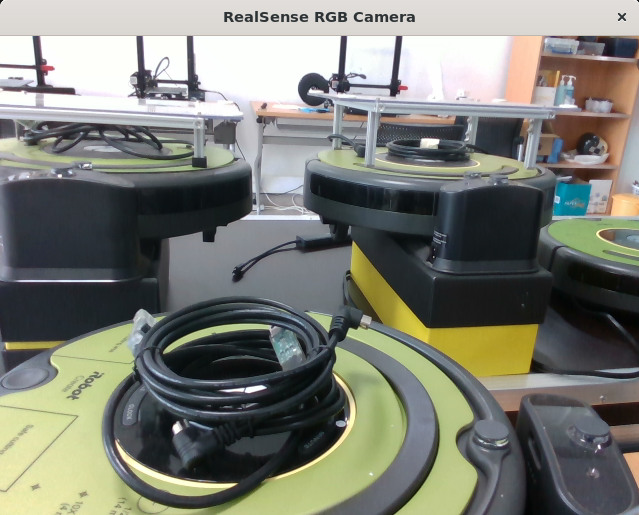
\includegraphics[width=\linewidth]{images/realsense_rgb.png}
		\caption{RealSense D435i RGB Camera Output.}
		\label{fig:realsense_rgb_image}
	\end{subfigure}
	\hfill
	\begin{subfigure}[b]{0.45\linewidth}
		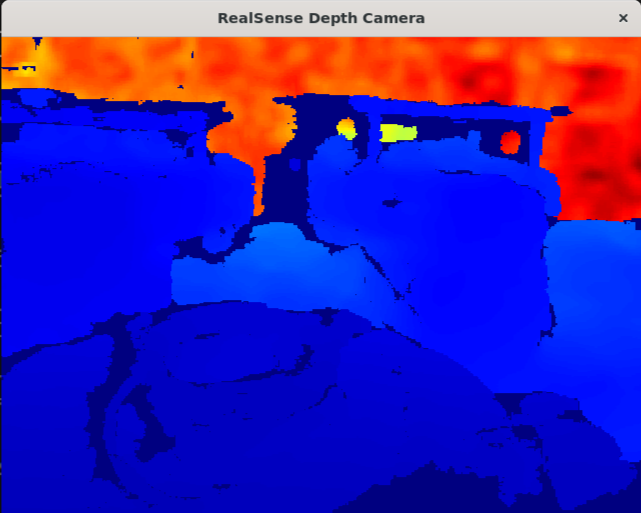
\includegraphics[width=\linewidth]{images/realsense_depth.png}
		\caption{RealSense D435i Depth Camera Output.}
		\label{fig:realsense_depth_image}
	\end{subfigure}
	\caption{Visual outputs from the Intel RealSense D435i camera. The RGB image shows the color view, while the depth image is rendered in grayscale.}
	\label{fig:realsense_camera_results}
\end{figure}


\subsection{Bottom, Front, and Stereo Camera Test}
The tests for the bottom, front, and stereo cameras are designed to evaluate the operational status of these essential sensors. 
By subscribing to the respective topics for each camera, the test confirms the continuous data publication, ensuring the 
cameras are functioning correctly. Utilizing the OpenCV library, the tests offer a visual confirmation by displaying images 
captured from the bottom, front, and stereo cameras. Each image is presented in a dedicated window, labeled with the corresponding 
sensor's name, allowing a visualization process. These images are displayed for 10 seconds. The test for these cameras will also log the 
width and height of the image.

It's important to note the distinction in camera availability between physical and simulator robots. Specifically, the stereo 
camera is exclusive to the physical robot, with no equivalent functionality in the simulator environment.

To initiate these tests, first, verify that the input file correctly enables the cameras by setting the key-value pairs for 
the front, bottom, and stereo cameras to \texttt{True}. Once confirmed, execute the designated command to launch the sensor tests on 
the robot.

The subsequent visualization results will provide a clear comparison between the capabilities of both the physical and simulator 
robots, highlighting the operational status and functionality of the tested cameras. This approach ensures a comprehensive assessment 
of the camera sensors, catering to both physical and simulated environments.

For more technical detail regarding the 2 RGB camera equipped on the robot, refer to the \href{http://doc.aldebaran.com/2-5/family/pepper_technical/video_2D_pep.html#d-camera-pepper}
{Pepper 2D camera technical detail}. Regarding the stereo camera, refer to the \href{http://doc.aldebaran.com/2-5/family/pepper_technical/video_Stereo_pep.html#stereo-camera-pepper}{Pepper 
stereo camera technical detail}.

\begin{figure}[ht]{}
	\centering
	\begin{subfigure}[b]{0.45\linewidth}
		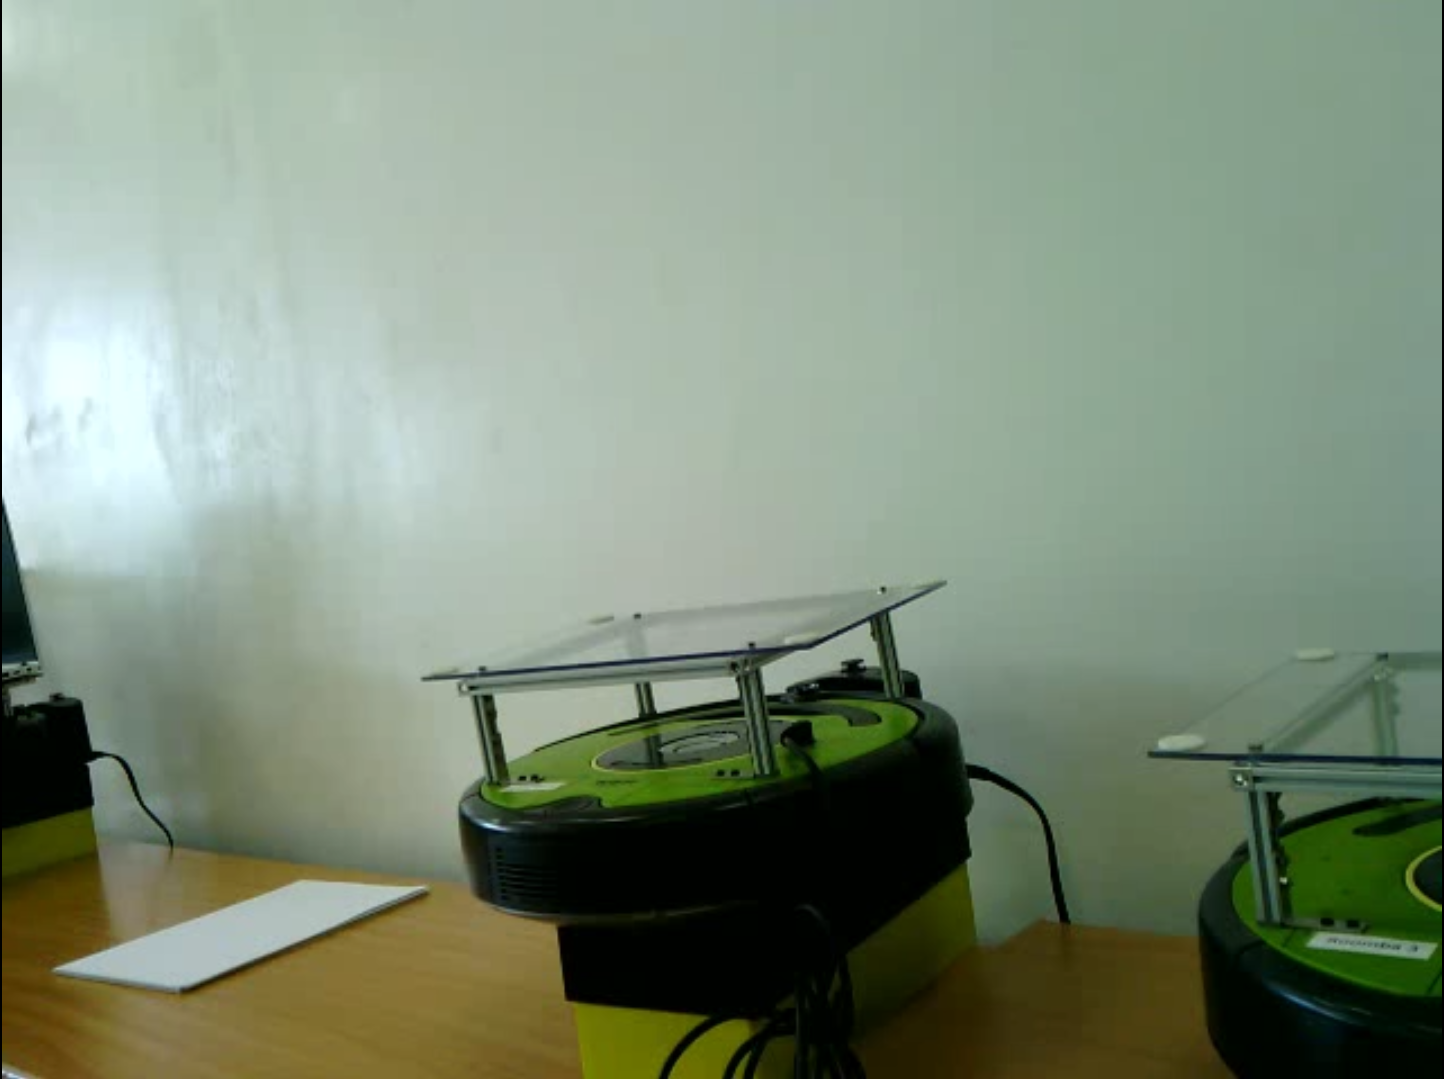
\includegraphics[width=\linewidth]{images/frontCamera.png}
		\caption{Front camera Image for Physical Robot.}
		\label{fig:Physical Front Camera Image}
	\end{subfigure}
	\hfill
	\begin{subfigure}[b]{0.45\linewidth}
		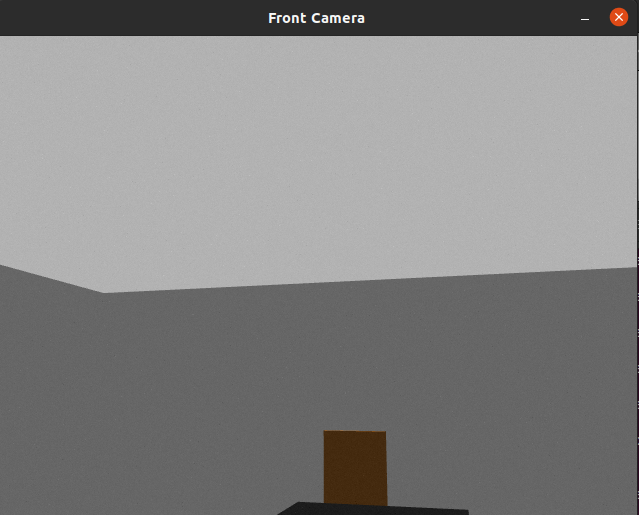
\includegraphics[width=\linewidth]{images/frontCameraSimulator.png}
		\caption{Front camera Image for the Simulator.}
		\label{fig:Simulator Front camera Image}
	\end{subfigure}
	\caption{Front Camera Image Result.}
	\label{fig:Front camera test}
\end{figure}

\begin{figure}[ht]
	  \centering
	  \begin{subfigure}[b]{0.45\linewidth}
		    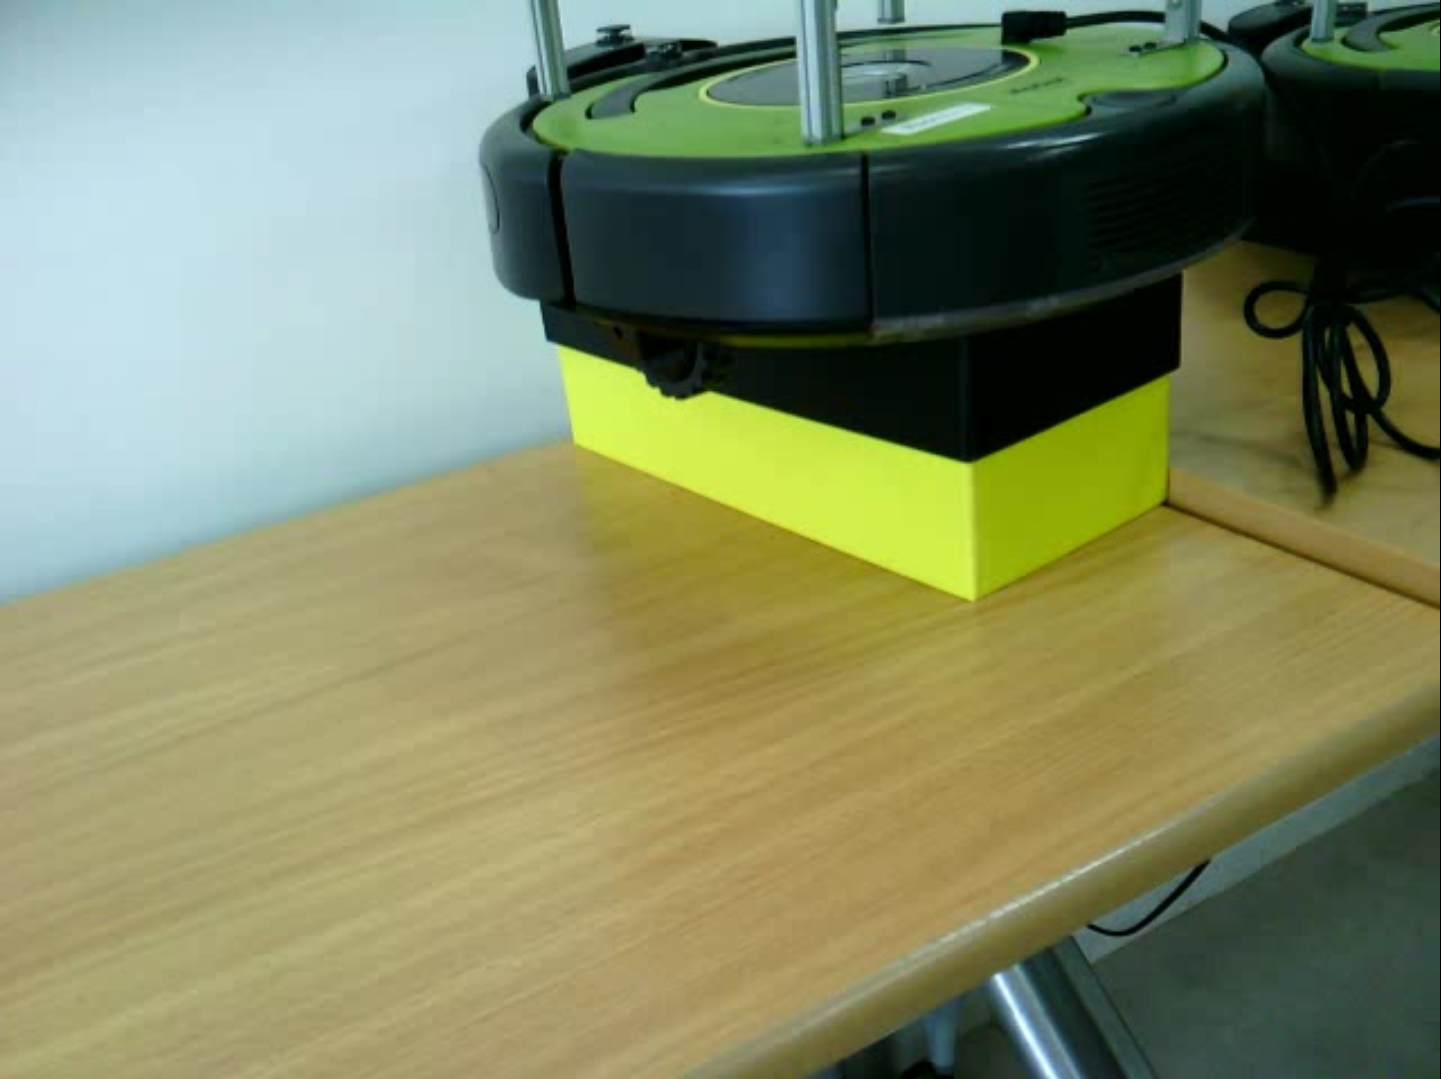
\includegraphics[width=\linewidth]{images/bottomCamera.png}
		    \caption{Bottom camera Image for Physical Robot.}
		    \label{fig:Physical Bottom camera}
		  \end{subfigure}
	  \hfill
	  \begin{subfigure}[b]{0.45\linewidth}
		    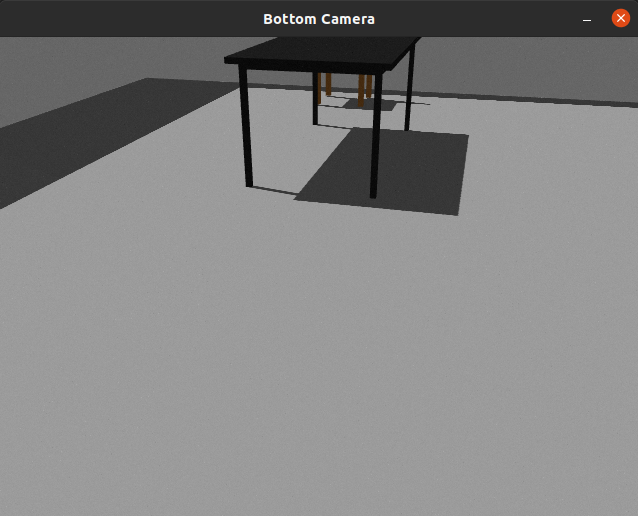
\includegraphics[width=\linewidth]{images/bottomCameraSimulator.png}
		    \caption{Bottom camera Image for the Simulator.}
		    \label{fig:Simulator Bottom camera}
		  \end{subfigure}
	  \caption{Bottom Camera Image Result}
	  \label{fig:Bottom camera test}
\end{figure}

As seen from the figure \ref{fig: Stereo Camera Image}, the stereo camera is displaying the pair of images captured by the 
two cameras side by side. 

\begin{figure}[!hbpt]
\centering
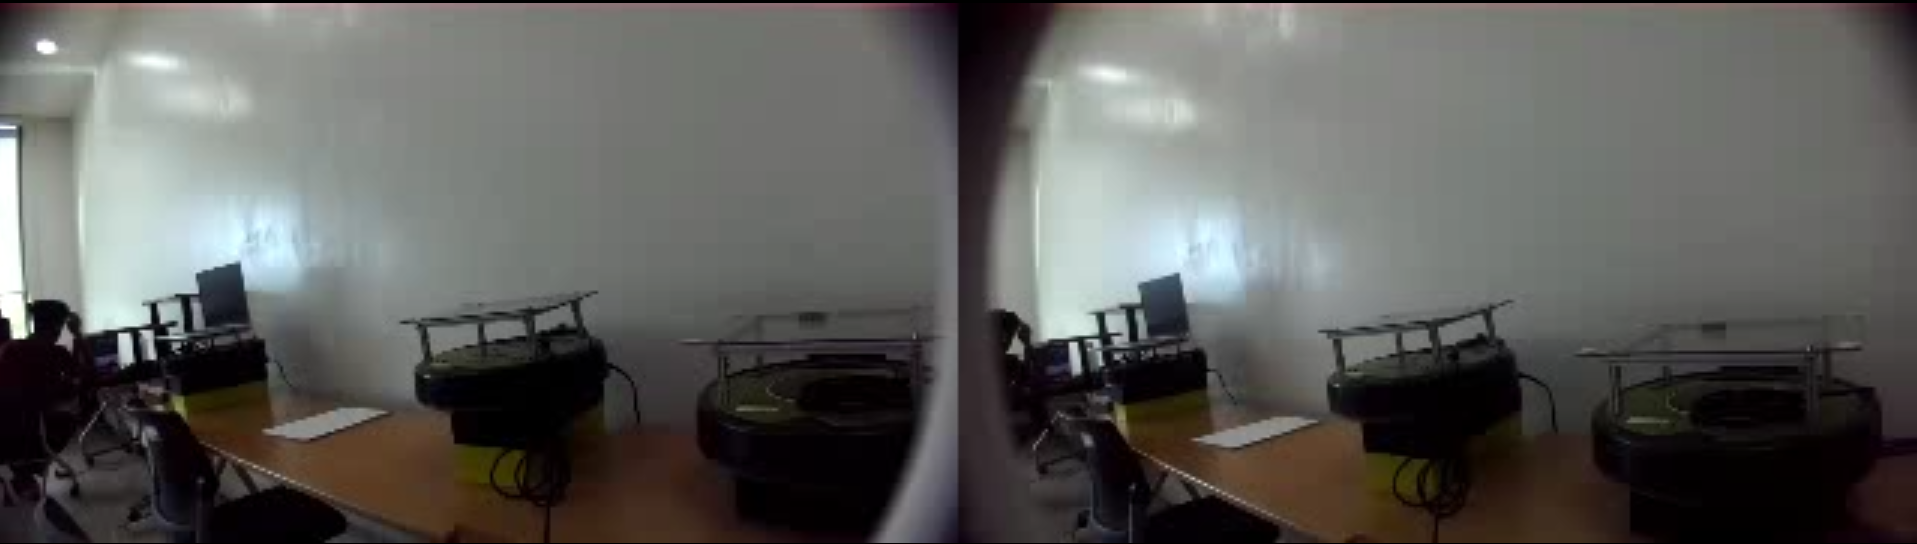
\includegraphics[scale=0.30]{images/stereoCamera.png}
\caption{Stereo Camera Image for the Physical Robot.}
\label{fig: Stereo Camera Image}
\end{figure}

The robot is equipped with dual cameras: a bottom camera and a front camera, capable of capturing RGB
format images that support multiple resolutions: \texttt{QQVGA(160x120)}, \texttt{QVGA(320x240)},
and \texttt{VGA(640x480)}. The selection of the desired resolution can be configured by modifying the file
\texttt{src/naoqi\_driver/share/boot\_config.json} settings. You can specify the resolution by using specifying
the integer accordingly to the once specified as \texttt{ "\_comment": "QQVGA = 0, QVGA = 1, VGA = 2"}. This allows
for flexible adaptation of image resolution based on the requirements of specific tasks or applications. The FPS 
parameter can be used to adjust the frame rate of the robot but as the number of sensor increase the frame rates
that could be achieved decrease. During the testing, the highest frame rate that could be achieved was 1.3 FPS.
However, after turning off most of the sensors except the front camera, the odometry, and the joint state, the frame rate
increased to 3.0 FPS. Therefore, this still could be limiting for some applications that require high frame rates.

\subsection{Depth Camera Test}
The depth camera test rigorously assesses the sensor's functionality by subscribing to its topic to confirm data flow 
and visualizing the output using the OpenCV library. Depth images are displayed in grayscale, with pixel intensity 
indicating the proximity to the camera, showcased in a window for 10 seconds. The depth sensor, which employs stereo camera technology, demonstrates limited efficacy when used at
distances greater than one meter. This limitation significantly impacts tasks such as environment map
generation (D5.5.3) that rely on Simultaneous Localization and Mapping (SLAM) techniques. The inherent
constraints of the depth camera's calibration process at extended ranges pose challenges to achieving
accurate and reliable results. Therefore, it is imperative to explore alternative methodologies to
fulfill the requirements of such tasks effectively.

Similarly to test the depth sensor for the physical robot or simulator, the user must set the key-value pair for the depth 
camera to \texttt{True} in the input file. Then execute sensorTest node to run the test.

As mentioned earlier, the depth camera is reconstructed from the stereo camera. For more technical details regarding the depth camera, 
refer to the \href{http://doc.aldebaran.com/2-5/family/pepper_technical/video_2D_pep.html#d-camera-pepper}{Pepper 3D camera technical detail}.

\begin{figure}[!hbpt]
    \centering
    \begin{subfigure}[b]{0.45\linewidth}
          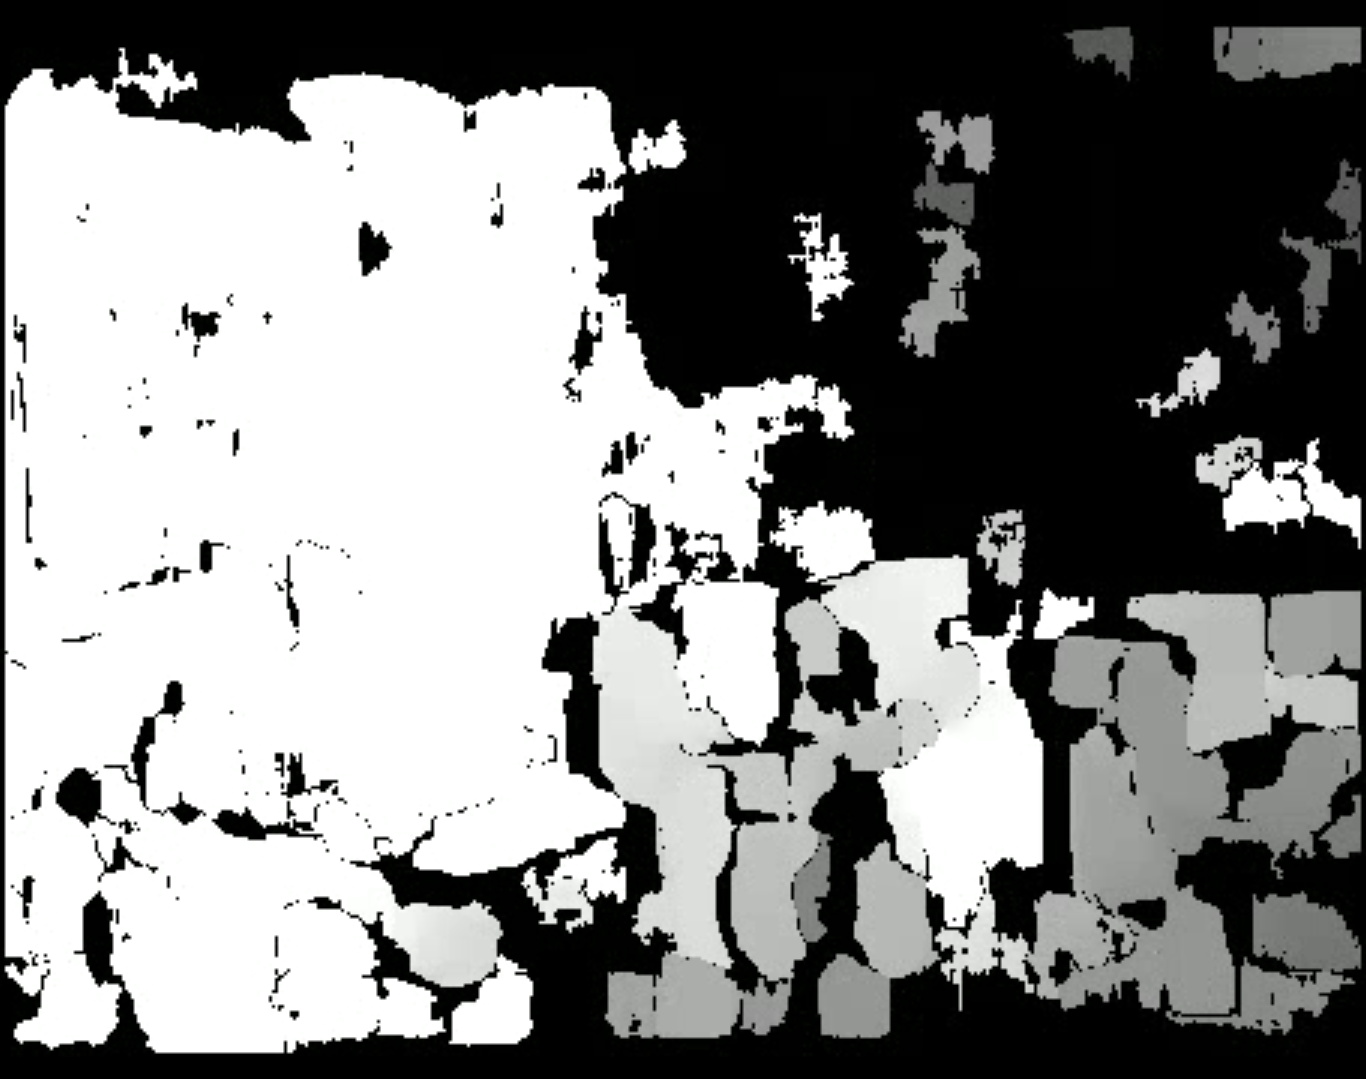
\includegraphics[width=\linewidth]{images/depthCamera.png}
          \caption{Depth Camera Image for Physical Robot.}
          \label{fig:Physical Depth Camera Image}
        \end{subfigure}
    \hfill
    \begin{subfigure}[b]{0.45\linewidth}
          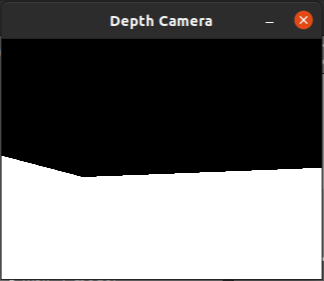
\includegraphics[width=\linewidth]{images/depthCameraSimulator.png}
          \caption{Depth Camera Image for Simulator.}
          \label{fig:Simulator Depth Camera Image}
        \end{subfigure}
    \caption{Depth Camera Result.}
    \label{fig:depth_camera_results} % Changed label to be unique
\end{figure}

The depth image shown in Figure \ref{fig:Physical Depth Camera Image} is an image captured by the stereo camera shown in Figure \ref{fig: Stereo Camera Image} which 
is converted to a depth image. Similarly, the Depth image for the simulator is shown in Figure \ref{fig:Simulator Depth Camera Image}.
However, for both the physical robot and simulator, the depth image doesn't provide a very clear image that can be used for
depth measurement.

\newpage

\subsection{Front and Back Sonar Test}
The sonar test is designed to capture and log the sensor's data both on the terminal for 
immediate observation and into an output file named \texttt{sensorTestOutput.dat} for references. 
During the test, the node will subscribe to the sonar topics for both the front and sonar sensors. 
To test the sonar sensor, the user must set the key-value pair for the front sonar and back sonar to \texttt{True} in the input file. 
Then execute the sensorTest node to run the test. The sonar sensor is capable of detecting objects within a range. Key metrics such 
as the range for object proximity is recorded. Upon receiving data, the test outputs a series 
of messages that detail:
% Create a Table to explain what each data point is (Frame ID, Field of View, Min Range, Max Range, Range)
\begin{longtable}[c]{|l|p{12cm}|}
	\caption{Sonar Test Output Data.} \label{tab:sonar_test_output}\\
	\hline
	\rowcolor{gray!30}
	\textbf{Data} & \textbf{Description} \\ \hline
	\endhead % header for subsequent pages
	\small{\texttt{Frame ID}} & \small{An identifier for the sensor data frame, ensuring that the data can be accurately correlated with its source and time of capture.} \\ \hline
	\small{\texttt{Field of View}} & \small{The angular extent of the observable world that the sonar sensor captures at any given moment.} \\ \hline
	\small{\texttt{Min Range}} & \small{The shortest distance at which the sonar sensor can reliably detect objects.} \\ \hline
	\small{\texttt{Max Range}} & \small{The furthest distance within which the sensor can effectively perceive objects.} \\ \hline
	\small{\texttt{Range}} & \small{The actual distance measured by the sonar sensor to the detected object, providing a directed indication of the object's proximity.} \\ \hline
\end{longtable}

Furthermore, please refer to the \href{http://doc.aldebaran.com/2-5/family/pepper_technical/sonar_pep.html#d-sonar-pepper}{Pepper sonar technical detail} for more technical detail 
such as frequency, resolution, vertical, and horizontal field of view.


\subsection{Laser Test}
The laser test is designed to capture and log the sensor's data both on the terminal for immediate observation and into an output file name \texttt{sensorTestOutput.dat} for references. 
During the test, the node will subscribe to the laser topic and record the range data. To test the laser sensor, the user must set the key-value pair for the laser sensor to \texttt{True} in the input file. 
Then execute the sensorTest node to run the test. The laser sensor is capable of detecting objects within a range. Upon receiving data, the test outputs a series of messages that detail:

\begin{longtable}[c]{|l|p{7cm}|}
	\caption{Laser Test Output Data.} \label{tab:laser_test_output}\\
	\hline
	\rowcolor{gray!30}
	\textbf{Data} & \textbf{Description} \\ \hline
	\endhead % header for subsequent pages
	\small{\texttt{Frame ID}} & \small{An identifier for the sensor data frame, ensuring that the data can be accurately correlated with its source and time of capture.} \\ \hline
	\small{\texttt{Start and End Angles of the Scan}} & \small{The scan covers an angular range field of view that is essential for comprehensive environmental scanning and obstacle detection.} \\ \hline
	\small{\texttt{Angular Distance between Measurements}} & \small{This metric reflects the sensor's angular resolution, determining the fineness of the scan and the sensor's ability to discern features.} \\ \hline
	\small{\texttt{Time between Measurements and Scans}} & \small{It indicates the time interval between consecutive measurements and scans, influencing the sensor's ability to capture dynamic environmental changes.} \\ \hline
	\small{\texttt{Minimum and Maximum Range Values}} & \small{The sensor is capable of detecting objects within a range defining the effective operational distance for reliable data acquisition.} \\ \hline
	\small{\texttt{Range Data}} & \small{This array of range data points captures the distances measured across the sensor's field of view, offering a dense dataset for analysis.} \\ \hline
\end{longtable}

For more technical details regarding the laser sensor, refer to the \href{http://doc.aldebaran.com/2-5/family/pepper_technical/laser_pep.html#d-laser-pepper}{Pepper laser technical detail} that shows 
the frame rate, horizontal and vertical field of view, and the resolution of the laser sensor.

\subsection{Microphone Test}
The microphone test is designed to capture and play the audio data from the robot's microphone. The test will record the audio data as \texttt{.wav} file and play the audio data. 
For the test, the user can speak or play a sound to the robot's microphone which is located at the top of the robot's head. The test will record the audio data for the four microphones for 10
seconds each as \texttt{.wav} file and saves the audio file in the \texttt{data} directory to do a system call to play the audio data. The user has the option to keep or delete the audio data. If the user wants to keep the audio data, the user can set the \texttt{deleteFile} key to \texttt{False} in the implementation file. 
Then compile the code and run the test. To test the microphone sensor, the user must set the key-value pair for the microphone sensor to \texttt{True} in the input file. 
Then execute the sensorTest node to run the test.

\vspace{0.5cm}

\begingroup
\tcbset{%
	noteshift/.store in=\mynote@shift,
	noteshift=0.8cm
}
\begin{tcolorbox}[nobeforeafter,
	enhanced,
	sharp corners,
	toprule=1pt,
	bottomrule=1pt,
	leftrule=0pt,
	rightrule=0pt,
	colback=yellow!20,
	left skip=\mynote@shift,
	right skip=\mynote@shift,
	overlay={\node[left] (mynotenode) at ([xshift=-\mynote@shift]frame.west) {\textbf{\textcolor{greenyellow}{Note:}}} ;},]
	The test is only available for the physical robot. The audio starts recording from the rearLeft microphone - rearRight microphone - frontLeft microphone - frontRight microphone.
	Ensure that the volume for your computer is set to a reasonable level to hear the audio recorded.
\end{tcolorbox}
\endgroup

The pepper robot has four microphones located at the top of the robot's head as shown in Figure \ref{fig:Microphone}. 
\begin{figure}[!hbpt]
	\centering
	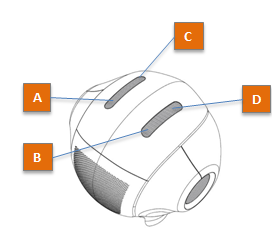
\includegraphics{images/Pepper_Microphone.png}
	\caption{Pepper's Microphone. Source: \href{http://doc.aldebaran.com/2-5/family/pepper_technical/microphone_pep.html}{Aldebaran}}
	\label{fig:Microphone}
\end{figure}

\newpage

% create a table to show the Part and Name of the microphone
\begin{longtable}[c]{|p{1.5cm}|p{6cm}|}
	\caption{Pepper Microphone Part and Name.} \label{tab:microphone_part_name}\\
	\hline
	\rowcolor{gray!30}
	\textbf{Part} & \textbf{Name} \\ \hline
	\endhead % header for subsequent pages
	\large{\texttt{A}} & \large{\texttt{MicroRL\_sensor}} \\ \hline
	\large{\texttt{B}} & \large{\texttt{MicroRR\_sensor}} \\ \hline
	\large{\texttt{C}} & \large{\texttt{MicroFL\_sensor}} \\ \hline
	\large{\texttt{D}} & \large{\texttt{MicroFR\_sensor}} \\ \hline
\end{longtable}

The custom message type \texttt{naoqi\_driver/AudioCustomMsg} records the audio data for the four microphones. The message type will have four data fields for the audio data representing 
the four microphones. 

The microphones are crucial for Deliverable D4.2.3 (Sound Detection and Localization) and Deliverable D4.3.2
(Speech Event) as it is used to perform automatic speech recognition. 

For more technical details regarding the microphone sensor, refer to the \href{http://doc.aldebaran.com/2-5/family/pepper_technical/microphone_pep.html}{Pepper microphone technical detail} 
which outlines the location of the four microphones, the frequency range, and the sensitivity of the microphones.

\subsection{Joint State Test}
The joint state test is designed to assess the functionality and accuracy of the joint state sensors 
by subscribing to the joint state topic and recording the joint state data. The sensor test will record
the status of each joint, including the position, velocity, and effort. The test will output the joint state
data to the terminal and save the joint state data to the output data file named \texttt{sensorTestOutput.dat}.
To test the joint state sensor, the user must set the key-value pair for the joint state sensor to \texttt{True} in the input file. 
Then execute the sensorTest node to run the test.

\newpage

Upon receiving data, the test outputs a series of messages that detail:

\begin{longtable}[c]{|l|p{12cm}|}
    \caption{Joint State Test Output Data.} \label{tab:joint_state_test_output}\\
    \hline
    \rowcolor{gray!30}
    \textbf{Data} & \textbf{Description} \\ \hline
    \endhead % header for subsequent pages
    \small{\texttt{Name}} & \small{The name of the joint for which the data is recorded, providing a clear reference for the specific joint being analyzed.} \\ \hline
    \small{\texttt{Position}} & \small{The current position of the joint, indicating the angle at which the joint is currently positioned. The position is measured in radians.} \\ \hline
    \small{\texttt{Velocity}} & \small{The velocity of the joint, reflecting the rate at which the joint is moving. The velocity is measured in radians per second.} \\ \hline
    \small{\texttt{Effort}} & \small{The effort exerted by the joint, representing the force or torque applied to the joint. The effort is measured in Newton-meters.} \\ \hline
\end{longtable}

\subsection{Odometry Test}
The odometry test is designed to assess the functionality and accuracy of the odometry sensor by subscribing to the odometry topic and recording the odometry data. 
The sensor test will record the odometry data, including the position, orientation, and linear and angular velocity. The test will output the odometry data to the terminal 
and save the odometry data to the output data file named \texttt{sensorTestOutput.dat}. 

To test the odometry sensor, the user must set the key-value pair for the odometry sensor to \texttt{True} in the input file. 
Then execute the sensorTest node to run the test.

Upon receiving data, the test outputs a series of messages that detail:
\begin{longtable}[c]{|l|p{10cm}|}
    \caption{Odometry Test Output Data.} \label{tab:odometry_test_output}\\
    \hline
    \rowcolor{gray!30}
    \textbf{Data} & \textbf{Description} \\ \hline
    \endhead % header for subsequent pages
    \small{\texttt{Timestamp}} & \small{The time at which the odometry data was recorded, providing a reference for the data's temporal context.} \\ \hline
    \small{\texttt{Frame of Reference}} & \small{The frame in which the odometry data is reported, ensuring that the data is accurately correlated with the robot's position and orientation.} \\ \hline
    \small{\texttt{Child Frame ID}} & \small{The ID of the frame that is moving, typically the base frame of the robot.} \\ \hline
    \small{\texttt{Pose}} & \small{The robot's position and orientation in the form of a pose message (geometry\_msgs/PoseWithCovariance), including both the pose and the covariance of the pose estimate.} \\ \hline
    \small{\texttt{Twist}} & \small{The robot's velocity in both linear and angular terms (geometry\_msgs/TwistWithCovariance), including the velocity and the covariance of the velocity estimate.} \\ \hline

\end{longtable}


\subsection{IMU Sensor Test}
The IMU sensor test is designed to assess the functionality and accuracy of the gyroscope and accelerometer sensors by subscribing to the IMU topic and recording the IMU data. 
The sensor test will record the IMU data, including the linear acceleration, angular velocity, and orientation. The test will output the IMU data to the terminal. Furthermore,
you can observe the IMU sensor publishes the data to two topics: \texttt{/naoqi\_driver/imu/base} and \texttt{/naoqi\_driver/imu/torso}. Both of the topics publish the IMU sensor 
data from different frames of reference. For the test, the sensor test will subscribe to the \texttt{/naoqi\_driver/imu/base} topic. 

To test the IMU sensor, the user must set the key-value pair for the IMU sensor to \texttt{True} in the input file. 
Then execute the sensorTest node to run the test.

The test will output the IMU data to the terminal. In addition, upon receiving data, the test outputs a series of messages that detail:


\begin{longtable}[c]{|l|p{10cm}|}
    \caption{IMU Sensor Test Output Data.} \label{tab:imu_sensor_test_output}\\
    \hline
    \rowcolor{gray!30}
    \textbf{Data} & \textbf{Description} \\ \hline
    \endhead % header for subsequent pages
    \small{\texttt{Orientation}} & \small{The sensor's current orientation in space, provided as a quaternion (x, y, z, w).} \\ \hline
    \small{\texttt{Angular Velocity}} & \small{The rate of rotation around the sensor's x, y, and z axes, typically in radians per second.} \\ \hline
    \small{\texttt{Linear Acceleration}} & \small{The acceleration vector along the sensor's x, y, and z axes, excluding gravity, usually in meters per second squared.} \\ \hline
    \small{\texttt{Covariance Matrices}} & \small{Estimates the noise and uncertainty of the orientation, angular velocity, and linear acceleration measurements, crucial for 
    algorithms that fuse sensor data for more accurate state estimation.} \\ \hline

\end{longtable}

For more technical details regarding the IMU sensor, refer to the \href{http://doc.aldebaran.com/2-5/family/pepper_technical/inertial_pep.html#d-inertial-pepper}{Pepper IMU technical detail}.
\subsection{Speech Test}
The speech test is designed to assess the functionality of speakers by publishing a speech command to the robot. The test will publish the speech in the form of a string message to the speech topic.
The text input provided for the speaker is \texttt{"This is the CSSR4Africa speaker test."}. 

To test the speech, the user must set the key-value pair for the speech to \texttt{True} in the input file. 
Then execute the sensorTest node to run the test.

\vspace{0.5cm}

\begingroup
\tcbset{%
    noteshift/.store in=\mynote@shift,
    noteshift=0.8cm
}
\begin{tcolorbox}[nobeforeafter,
    enhanced,
    sharp corners,
    toprule=1pt,
    bottomrule=1pt,
    leftrule=0pt,
    rightrule=0pt,
    colback=yellow!20,
    left skip=\mynote@shift,
    right skip=\mynote@shift,
    overlay={\node[left] (mynotenode) at ([xshift=-\mynote@shift]frame.west) {\textbf{\textcolor{greenyellow}{Note:}}} ;},]
    The test is only available for the physical robot. Ensure that the volume of the robot is set to a reasonable level to hear the speech.
\end{tcolorbox}

For more technical details regarding the speaker, refer to the \href{http://doc.aldebaran.com/2-5/family/pepper_technical/speaker_pep.html#d-speaker-pepper}{Pepper speaker technical detail}.


\newpage
\bibliographystyle{unsrt}
%================================================================
\bibliography{cognitive_systems.bib}                                     % REPLACE with correct filename
\addcontentsline{toc}{section}{References}

\pagebreak
\section*{Principal Contributors}
%===============================================================
\label{contributors}
\addcontentsline{toc}{section}{Principal Contributors}
The main authors of this deliverable are as follows (in alphabetical order).
\blank
~
\blank
Yohannes Haile, Carnegie Mellon University Africa.\\    % REPLACE with correct name and affiliation
David Vernon, Carnegie Mellon University Africa. \\                                                                           % REMOVE
 

  
\newpage
\section*{Document History}
%================================================================
\addcontentsline{toc}{section}{Document History}
\label{document_history}

\begin{description}

\item [Version 1.0]~\\
First draft. \\
Yohannes Haile. \\                                     % REPLACE with correct name
26 March 2024.                                         % REPLACE with correct date

\item [Version 1.1]~\\
Fixed error changed actuator test to sensor test on Page 11.\\
Fixed repetition ``All of the sensors ..." on Page 7.\\
Fixed the sensor test diagram flow chart.\\	
Changed the title from Source Code \textrightarrow{} File Organization.\\
Added the real sense camera in the test.\\
Yohannes Haile. \\                                     % REPLACE with correct name
31 May 2025.                                         % REPLACE with correct date


\end{description}

\end{document}

